\cotefile{1}
\scanpage{93}

\uline{Th 4} (\uline{troisième th. de convexité dans les espaces de Hilbert})

\reversemarginpar
\margin{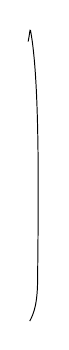
\begin{tikzpicture}[x=1cm,y=1cm]
\draw[line width=.35pt] (0,3.55)..controls (.02,3.64) and (.02,3.72)..(.03,3.69)..controls (.15,3.05) and (.13,1.55)..(.12,.54)..controls (.12,.22) and (.07,.09)..(.02,0);
\end{tikzpicture}}
\normalmarginpar
Soient $E,F$ deux espaces de Hilbert, $u,v$ deux opérateurs compacts de $E$ dans $F$, soit enfin $\varphi\inserted{(s_1,\mathord{-}s_n)}$ une fonction \deleted{\unsure{continue|convexe} symétrique}\inserted{convexe symétrique \unsure{croiss.|croissante} \deleted{et \unsure{épist.}}} de $n$ arguments $s_i\geq0$, \deleted{telle que $\unsure{f(e^{t_1},\quad e^{t_n})|f e^{t_1},\quad e^{t_n})}$ soit fonction convexe de $(\unsure{h|t_i})\in R^n$. Alors,}\inserted{Alors}

\[
\text{(41)}\qquad
\varphi(\rho_1(u+v),\mathord{-}\,\mathord{-},\rho_n(u+v))\leq
\varphi(\rho_1(u)+\rho_1(v),\mathord{\cdot}\,\mathord{-},\rho_n(u)+\rho_n(v))
\]

En effet, c'est un cas particulier du Th. 1, 1\uuline{°}, hypothèse c, compte tenu des formules du N\uline{°} 1.

\begingroup
\setbox0=\vbox{\hsize=\linewidth
\noindent\deleted{\uline{Corollaire} \unsure{Soit|Soient|Etant} $u$ et $v$ étant comme ci-dessus, soit $\varphi(s)$ une fonction convexe \inserted{\unsure{croiss.|croissante}} de $s\geq0$, alors on a pour tout entier $n>0$}
\[
\deleted{\text{(42)}\qquad\sum_1^n\varphi(\rho_i(u+v))\leq\sum_1^n\varphi(\rho_i(u)+\rho_i(v))}
\]}
\dimen0=\wd0\advance\dimen0 by4pt
\dimen2=\ht0\advance\dimen2 by-2pt
\dimen4=\dp0\advance\dimen4 by2pt
\dimen6=\ht0\advance\dimen6 by-12pt
\noindent\rlap{\begin{tikzpicture}[overlay,baseline=0pt]
\draw[line width=.35pt] (-3pt,\the\dimen2)..controls (-2pt,\the\dimen6) and (-3pt,4pt)..(0pt,-\the\dimen4)--(9pt,-\the\dimen4);
\draw[line width=.35pt] (\the\dimen0,\the\dimen6)..controls (\the\dimen0,12pt) and (\the\dimen0,4pt)..(\the\wd0,-\the\dimen4);
\end{tikzpicture}}\box0
\endgroup

Nous serons surtout \unsure{intéressé|intéressés} par le

\uline{Corollaire} 1 Soient \deleted{$u$ et $v$ comme ci-dessus,}\inserted{$E$ et $F$ deux espaces de Hilbert,} et soit $N$ \uline{une norme de Schatten} sur $R^n$, \deleted{alors la quantité} posons, pour \deleted{tout} opérateur compact $u$ de $E$ dans $F$

\[
\text{(4\unsure{3|2})}\qquad
\lVert u\rVert_N=N(\rho_1(u),\mathord{-}\rho_n(u))
\]

Alors on a

\begin{center}
\(\text{(44)}\qquad\)
\begingroup
\setbox0=\hbox{$\lVert u+v\rVert_N\leq\lVert u\rVert_N+\lVert v\rVert_N$}
\dimen0=\wd0\advance\dimen0 by6pt
\dimen2=\ht0\advance\dimen2 by5pt
\dimen4=\dp0\advance\dimen4 by4pt
\dimen6=\dimen2\advance\dimen6 by-3pt
\leavevmode\hspace{3pt}
\rlap{\raise\dimen2\hbox{$\deleted{\lVert\lambda u\rVert_N=|\lambda|\lVert u\rVert_N}$}}
\rlap{\begin{tikzpicture}[overlay,baseline=0pt]
\draw[red,line width=.8pt] (-3pt,\the\dimen2)--(\the\wd0,\the\dimen2)..controls (\the\dimen0,\the\dimen2) and (\the\dimen0,\the\dimen6)..(\the\wd0,1pt);
\draw[red,line width=.8pt] (-3pt,\the\dimen2)--(-3pt,-\the\dimen4)--(\the\wd0,-\the\dimen4)--(\the\wd0,-1pt);
\end{tikzpicture}}
\box0\hspace{6pt}
\endgroup
\end{center}

\deleted{et $\unsure{u\to\lVert u\rVert_N}$ \unsure{définit|est donc} \illegible{2} \unsure{$u\in L_0(E,F)$|$(L_0(E,F))$} \unsure{tels que|sous-espace} \unsure{Si} $N$ est une norme de \unsure{Schatten} \unsure{sur} $R\quad\unsure{R_+^{(n)}|R^{(N)}|R^{(\underline N)}}$}

En effet, $N(s_1,\mathord{-}s_n)$ pour $s_i\geq0$ satisfait aux conditions de (41), on a donc

\[
N(\rho_1(u+v),\mathord{-},\rho_i(u+v))\leq
N(\rho_1(u)+\rho_1(v),\mathord{\cdot}\,\mathord{-},\rho_i(u)+\rho_i(v))
\]

et le second \unsure{$=$b|$\bar m$b} est majoré par $N(\rho_1(u),\mathord{-},\rho_n(u))+N(\rho_1(v),\mathord{-},\rho_n(v))$ puisque $N$ est une norme, d'où (44).

En particulier

\uline{Corollaire 1} \deleted{\unsure{Pour les|Soient}} si $u,v\in L_0^{\unsure{p}}(E,F)$, \deleted{\unsure{alors|et si}} \unsure{cf|(f} $1\leq p\leq+\infty$)) $\mathord{\cdot}\,\mathord{-}\,.$ pour \deleted{\unsure{tout}} \inserted{entier $n>0$}

\[
\deleted{\lVert u+v\rVert_p\leq}
\]
\[
\text{(45)}\qquad
\left(\sum_1^n(\rho_i(u+v))^p\right)^{1/p}\leq
\left(\sum_1^n\rho_i(u)^p\right)^{1/p}+
\left(\sum_1^n\rho_i(v)^p\right)^{1/p}
\]

donc \unsure{par|en} \deleted{\unsure{$(N$|$(\varphi$|(passant|(passage} \illegible{3}} \deleted{$\unsure{\sum}$}

\begin{center}
\(\text{(46)}\qquad\)
\begingroup
\setbox0=\hbox{$\lVert u+v\rVert_p\leq\lVert u\rVert_p+\lVert v\rVert_p$}
\dimen0=\wd0\advance\dimen0 by7pt
\dimen2=\ht0\advance\dimen2 by5pt
\dimen4=\dp0\advance\dimen4 by3pt
\dimen6=\dimen2\advance\dimen6 by2pt
\dimen8=\dimen0\advance\dimen8 by12pt
\leavevmode\hspace{3pt}
\rlap{\begin{tikzpicture}[overlay,baseline=0pt]
\draw[red,line width=.5pt] (-13pt,\the\dimen6)--(\the\dimen8,\the\dimen6);
\draw[red,line width=.5pt] (-3pt,\the\dimen2)--(-3pt,-\the\dimen4)--(\the\dimen0,-\the\dimen4)--(\the\dimen0,\the\dimen2);
\end{tikzpicture}}
\box0\hspace{7pt}
\endgroup
\end{center}

\reversemarginpar
\margin{94}
\normalmarginpar
